%!TEX root = ../template.tex
%%%%%%%%%%%%%%%%%%%%%%%%%%%%%%%%%%%%%%%%%%%%%%%%%%%%%%%%%%%%%%%%%%%%
%% chapter4.tex
%% NOVA thesis document file
%%
%% Chapter with lots of dummy text
%%%%%%%%%%%%%%%%%%%%%%%%%%%%%%%%%%%%%%%%%%%%%%%%%%%%%%%%%%%%%%%%%%%%

\typeout{NT FILE chapter4.tex}%

\chapter{Methodology}
\label{cha:methodology}


\FloatBarrier
\section{WhyRel: what we used and what we did different}
\label{sec:whyrel_diff}




\FloatBarrier
\section{bip2ml}
\label{sec:bip2ml}

\begin{figure}[htbp]
  \centering
  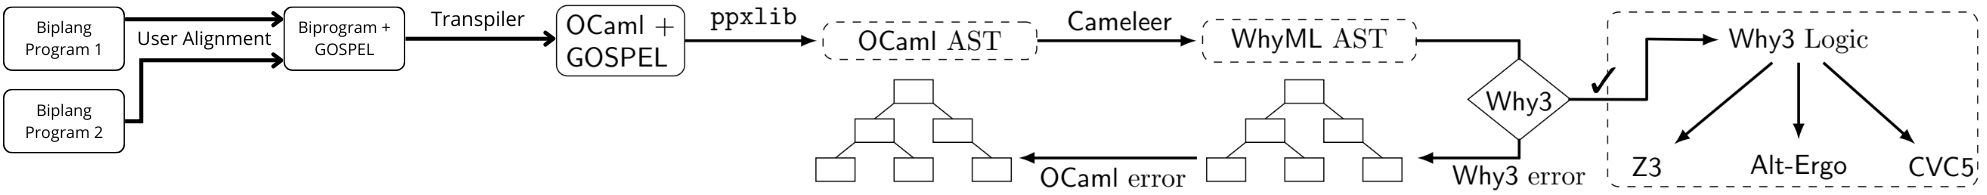
\includegraphics[max width=\textwidth]{transpiler+cameleer_pipeline}
  \caption{Architecture and verification pipeline of our transpiler and Cameleer}
  \label{fig:transpiler_cameleer_pipeline}
\end{figure}

\begin{figure}[htbp]
  \centering
  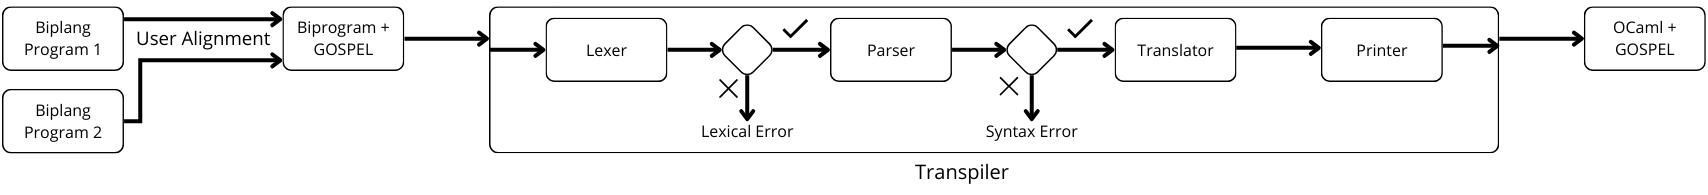
\includegraphics[max width=\textwidth]{transpiler_pipeline}
  \caption{Architecture and pipeline of bip2ml}
  \label{fig:transpiler_pipeline}
\end{figure}


\FloatBarrier
\subsection{Language Definition}
\label{subsec:lang_def}

We now present the grammar of our language.
The syntaxes of the most relevant rules are given by the following extended BNF definition.
Note that Biplang's keywords are written in bold.

\begin{lstlisting}[mathescape, basicstyle=\ttfamily, columns=flexible,
                    emph={type, and, let, rec, if, then, else, mod, in, for, while, do, done, to, begin, end, assert, match, with, of, open, include},
                    emphstyle=\ttfamily\bfseries]
file ::= decl*

decl ::= 
            | def
            | spec
            | typedef

spec ::= { loc: location; text: string; }

typedef ::=
              | type id = payload (and typedef)?
              | type id = $\overrightarrow{constructor}$ (and typedef)?

payload ::= 
              | $\overrightarrow{bt}$
              | $\overrightarrow{id}$

constructor ::= idc * payload?

def ::= let rec? id ($\overrightarrow{parameter}$) : fun_ret? = $\overrightarrow{expr}$ spec

expr ::=
            | ()
            | (e)
            | c
            | id
            | -e
            | $\neg$ e
            | ref e 
            | !e
            | e + e
            | e - e
            | e * e
            | e / e
            | e mod e
            | e = e
            | e <> e
            | e < e
            | e $\leq$ e
            | e > e
            | e $\geq$ e
            | e == e
            | e != e
            | e && e
            | e || e 
            | let id = e in $\overrightarrow{e}$
            | if $e_1$ then $e_2$ else $e_3$
            | for id = $e_1$ to $e_2$ do spec? $e_3$ done 
            | while $e_1$ do spec? $e_2$ done 
            | id := e
            | assert (e)
            | match id with ($\overrightarrow{case}$)
            | ($\overrightarrow{e}$)
            | idc ($\overrightarrow{e}$)
            | fun_id ($\overrightarrow{e}$)
            | Module_id.fun_id ($\overrightarrow{e}$)
            | def in e
            
            $\emph{arrays}$
            | [| $\overrightarrow{e}$ |]
            | id.(e)
            | id.($e_1$) <- $e_2$

            $\emph{lists}$
            | [ $\overrightarrow{e}$ ]
            | e :: [ $\overrightarrow{e}$ ]
            | e @ [ $\overrightarrow{e}$ ]

            $\emph{introduced by BipLang}$
            | $e_1$ <|> $e_2$ $\emph{(pipe)}$
            | $\lfloor e \rfloor$ $\emph{(floors)}$
            | while $e_1$ <|> $e_2$ . $e_3$ <|> $e_4$ do spec? $e_5$ done
            $\emph{(conditionally aligned loops)}$

c ::=
        | None
        | int
        | bool
        | string

\end{lstlisting}

explicar: id, idc, bt, at, payload, constructor, parameter, fun\_ret, c, case

FALAR DAS DIFERENÇAS E SEMELHANÇAS ENTRE BIPLANG E OCAML


\FloatBarrier
\subsection{Translator}
\label{subsec:translator}


\FloatBarrier
\subsubsection{Printer}
\label{subsubsec:printer}


\FloatBarrier
\subsection{Syntax Highlighter}
\label{subsec:syntax_highlighter}




\iffalse
Proving the equivalence of two different OCaml programs can be a hard task, depending on the complexity and size of said programs.
Therefore, we implemented a small set of simple programs that show two different ways of establishing program equivalence.
The first one relies on including a post-condition that states that the result of program P$_1$ is equal to the result of program P$_2$ for the same input.
The second way uses product programs, where we present the source and the transformed programs.
Then, we apply \hyperref[fig:product_construction_equal_struct]{these} rules to create the corresponding product program, which can be proven with standard verification.

\FloatBarrier
\section{Simple equivalence proofs}
\label{sec:results_eq_proofs}

In this section, we present the functional and imperative implementations of each algorithm.
We also compare the specification of each implementation, pointing the similarities and differences.
All of the following programs have been verified using \hyperref[sec:cameleer]{Cameleer} and the information in the tables was provided by \hyperref[sec:why3]{Why3}.


\subsection{Factorial}
\label{sub:factorial}

Both functional and imperative implementations of the factorial have only one pre condition \emph{n >= 0}.
They differ, however, in the post condition, which is \emph{result = fact n} in the case of the imperative implementation and non-existent in the case of the functional implementation.
Moreover, the functional implementation has a variant \emph{n}, while the imperative implementation has an invariant, \emph{!res = fact (i-1)}. 

\bigskip
\newcommand{\provername}[1]{\cellcolor{yellow!25}
\begin{sideways}\textbf{#1}~~\end{sideways}}
\newcommand{\explanation}[1]{\cellcolor{yellow!13}lemma \texttt{#1}}
\newcommand{\transformation}[1]{\cellcolor{yellow!13}transformation \texttt{#1}}
\newcommand{\subgoal}[2]{\cellcolor{yellow!13}subgoal #2}
\newcommand{\valid}[1]{\cellcolor{green!13}#1}
\newcommand{\unknown}[1]{\cellcolor{red!20}#1}
\newcommand{\invalid}[1]{\cellcolor{red!50}#1}
\newcommand{\timeout}[1]{\cellcolor{red!20}(#1)}
\newcommand{\outofmemory}[1]{\cellcolor{red!20}(#1)}
\newcommand{\noresult}{\multicolumn{1}{>{\columncolor[gray]{0.8}}c|}{~}}
%\newcommand{\failure}{\cellcolor{red!20}failure}
\newcommand{\highfailure}{\cellcolor{red!50}FAILURE}
    
\begin{minipage}{\linewidth}
\begin{gospel}
  (*@ function rec fact (n: integer) : integer =
  if n = 0 then 1 else n * fact (n-1) *)
  (*@ requires n >= 0 
    variant n *)
\end{gospel}
\end{minipage}

\begin{minipage}{\linewidth}
\begin{ocamlenv}
  let fact_iter (n: int) : int =
    if n <= 1 then 1
    else
      begin 
        let res = ref 1 in
        for i = 2 to n do
          (*@ invariant !res = fact (i-1) *)
          res := !res * i
        done;
        !res
      end
  (*@ result = fact_iter n
    requires n >= 0 
    ensures result = fact n *)
\end{ocamlenv}
\end{minipage}

Regarding the proof of both the implementations of the factorial, Z3 was able to discard all of the verification conditions (VCs) automatically.
Furthermore, this SMT solver took a quarter of a second to complete the whole proof, verifying the functional implementation in 0.08 seconds and the imperative implementation in 0.17 seconds.

\begin{table}[!h]
\begin{center}
\begin{tabular}{|l|l|l|l|c|}
  \hline \multicolumn{2}{|c|}{Proof obligations } & \provername{Z3 4.13.0} \\ 
  \hline
  \explanation{VC for fact}  & \explanation{variant decrease} & \valid{0.03} \\ 
  \cline{2-3}
    & \explanation{precondition} & \valid{0.05} \\ 
  \hline
  \explanation{VC for fact\_iter}  & \explanation{postcondition} & \valid{0.04} \\ 
  \cline{2-3}
    & \explanation{loop invariant init} & \valid{0.05} \\ 
  \cline{2-3}
    & \explanation{loop invariant preservation} & \valid{0.04} \\ 
  \cline{2-3}
    & \explanation{postcondition} & \valid{0.01} \\ 
  \cline{2-3}
    & \explanation{VC for fact\_iter} & \valid{0.03} \\ 
  \hline 
\end{tabular}
\caption{Factorial implementations verification results.}
\end{center}
\end{table}


\subsection{Fibonacci}
\label{sub:fibonacci}

Both functional and imperative implementations of the factorial have only one pre condition \emph{n >= 0}.
They differ, however, in the post condition, which is \emph{result = fib n} in the case of the imperative implementation and non-existent in the case of the functional implementation.
Moreover, the functional implementation has a variant \emph{n}, while the imperative implementation has two invariants, \emph{!prev = fib (i-2)} and \emph{!res = fib (i-1)}. 

\begin{minipage}{\linewidth}
\begin{gospel}
  (*@ function rec fib (n: integer) : integer =
  if n <= 1 then n else fib (n-1) + fib (n-2) *)
  (*@ requires n >= 0 
    variant n *)
\end{gospel}
\end{minipage}

\bigskip

\begin{minipage}{\linewidth}
\begin{ocamlenv}
  let fib_iter (n: int) : int =
    if n <= 1 then n
    else
      begin
        let prev = ref 0 in 
        let res = ref 1 in
        let temp = ref 1 in

        for i = 2 to n do
          (*@ invariant !prev = fib (i-2)
            invariant !res = fib (i-1) *)
          temp := !res;
          res := !res + !prev;
          prev := !temp;
        done;

        !res
      end
  (*@ result = fib_iter n
    requires n >= 0 
    ensures result = fib n *)
\end{ocamlenv}
\end{minipage}

\bigskip

Using Z3 as we did with the factorial, we were able to prove the correctness of both implementations without any human intervention, taking a total of 0.3 seconds.
Besides that, the SMT solver spent 0.13 seconds verifying the functional implementation and 0.17 seconds verifying the imperative implementation.

\begin{table}[!h]
  \begin{center}
  \begin{tabular}{|l|l|l|l|c|}
    \hline \multicolumn{2}{|c|}{Proof obligations } & \provername{Z3 4.13.0} \\ 
    \hline
    \explanation{VC for fib}  & \explanation{variant decrease} & \valid{0.03} \\ 
    \cline{2-3}
      & \explanation{precondition} & \valid{0.03} \\ 
    \cline{2-3}
      & \explanation{variant decrease} & \valid{0.03} \\ 
    \cline{2-3}
      & \explanation{precondition} & \valid{0.04} \\ 
    \hline
    \explanation{VC for fib\_iter}  & \explanation{postcondition} & \valid{0.03} \\ 
    \cline{2-3}
      & \explanation{loop invariant init} & \valid{0.02} \\ 
    \cline{2-3}
      & \explanation{loop invariant init} & \valid{0.03} \\ 
    \cline{2-3}
      & \explanation{loop invariant preservation} & \valid{0.02} \\ 
    \cline{2-3}
      & \explanation{loop invariant preservation} & \valid{0.03} \\ 
    \cline{2-3}
      & \explanation{postcondition} & \valid{0.01} \\ 
    \cline{2-3}
      & \explanation{VC for fib\_iter} & \valid{0.03} \\ 
    \hline 
  \end{tabular}
  \caption{Fibonacci implementations verification results.}
\end{center}
\end{table}


\section{Equivalence proofs using product programs}
\label{sec:results_eq_proofs_pp}

In this section, we present a program and a slightly different version.
Then we combine them using the technique of product programs, more specifically, \hyperref[fig:product_construction_equal_struct]{these} rules. 
Finally, we verified those product programs using the \hyperref[sec:why3]{Why3} tool.
The results present on the tables were generated by that tool.
All the code is written in WhyML.


\subsection{Program based on assignments}
\label{sub:results_assignments}

The (original) program is based on only two assignment instructions: \emph{y := x + 1;} and \emph{z := y + 1;}.
Despite being a very simple example, it is enough to show the usage of the product construction rules in practice.

To make the programs separable, we renamed \emph{x}, \emph{y} and \emph{z} in the original program to \emph{x1}, \emph{y1} and \emph{z1} and in the transformed program to \emph{x2}, \emph{y2} and \emph{z2}.
The product program establishes that, if the values of the variables \emph{x1} and \emph{x2} are the same before the function \emph{product} starts, it is guaranteed that \emph{y1 = y2} and \emph{z1 = z2}.
And, since there is no assignment to any of the x-components, \emph{x1 = x2} will also be true if the pre-condition is respected.

There was no need for human intervention in verifying the product program, as the SMT solver Z3 completed the proof in under a second.

\begin{figure}
  \centering
  \begin{subfigure}[b]{0.45\textwidth}
    \begin{minipage}[t]{\linewidth}
      \textbf{Original program}
      \begin{whylang}
        use int.Int
      
        val ref x : int
        val ref y : int
        val ref z : int
      
        let original ()
          =
          y <- x + 1; 
          z <- y + 1;
      \end{whylang}
    \end{minipage}
  \end{subfigure}
  \hfill
  \begin{subfigure}[b]{0.45\textwidth}
    \begin{minipage}[t]{\linewidth}
      \textbf{Transformed program}
      \begin{whylang}
        use int.Int
      
        val ref x : int
        val ref y : int
        val ref z : int
      
        let transformed ()
          =
          z <- x + 2; 
          y <- z - 1;
      \end{whylang}
    \end{minipage}
  \end{subfigure}
  \hfill
  \begin{subfigure}[b]{0.9\textwidth}
    \begin{minipage}[t]{\linewidth}
      \textbf{Product program}
      \begin{whylang}
        use int.Int
      
        val ref x1 : int
        val ref x2 : int
        val ref y1 : int
        val ref y2 : int
        val ref z1 : int
        val ref z2 : int
      
        let product ()
          requires { x1 = x2 }
          ensures { y1 = y2 }
          ensures { z1 = z2 }
          =
          y1 <- x1 + 1; 
          z2 <- x2 + 2;
          z1 <- y1 + 1;
          y2 <- z2 - 1;
      \end{whylang}
    \end{minipage}
  \end{subfigure}
  \caption{Program based on assignments.}
  \label{fig:pp_ex_assignments}
\end{figure}

\begin{table}[!h]
  \begin{center}
  \begin{tabular}{|l|l|l|l|c|}
    \hline \multicolumn{2}{|c|}{Proof obligations } & \provername{Z3 4.13.0} \\ 
    \hline
    \explanation{VC for product}  & \explanation{postcondition} & \valid{0.01} \\ 
    \cline{2-3}
    & \explanation{postcondition} & \valid{0.00} \\ 
    \hline 
  \end{tabular}
  \caption{Program based on assignments verification results.}
  \end{center}
\end{table}  


\FloatBarrier
\subsection{Program with a while loop}
\label{sub:results_while}

This program, already mentioned \hyperref[fig:induction_var_strength_red]{before}, is slightly more complex than the example before, as this one features a while loop.
The optimization here comes from the fact that, for a computer, a multiplication is more expensive than an addition, especially when performed inside a loop.
This is called induction variable strength reduction.

The product program does not need a pre-condition, but its post.condition states that \emph{x = x'} at the end of the execution.
So, how is this achieved?
Well, with one variant to prove termination and three invariants to guarantee the post-condition; one of them is the exact same comparison (\emph{invariant \{x = x'\}}).

The proof was completed automatically by Z3 and the total duration was 0.16 seconds.

\begin{figure}
  \centering
  \begin{subfigure}[b]{0.45\textwidth}
    \begin{minipage}[t]{\linewidth}
      \textbf{Original program}
      \begin{whylang}
        use int.Int

        let source (b c n: int) : (x: int)
        = let ref i = 0 in
          let ref j = 0 in
          let ref x = 0 in
          while i < n do
            j <- i * b + c;
            x <- x + j;
            i <- i + 1;
          done;
          x
      \end{whylang}
    \end{minipage}
  \end{subfigure}
  \hfill
  \begin{subfigure}[b]{0.45\textwidth}
    \begin{minipage}[t]{\linewidth}
      \textbf{Transformed program}
      \begin{whylang}
        use int.Int

        let transformed (b c n: int) : (x': int)
        = let ref i' = 0 in
          let ref j' = c in
          let ref x' = 0 in
          while i' < n do
            x' <- x' + j';
            j' <- j' + b;
            i' <- i' + 1
          done;
          x'
      \end{whylang}
    \end{minipage}
  \end{subfigure}
  \hfill
  \begin{subfigure}[b]{0.9\textwidth}
    \begin{minipage}[t]{\linewidth}
      \textbf{Product program}
      \begin{whylang}
        use int.Int

        let product (b c n: int) : (x: int, x': int)
          ensures { x = x' }
        = let ref i = 0 in
          let ref i' = 0 in
          let ref j = 0 in
          let ref j' = c in
          let ref x = 0 in
          let ref x' = 0 in
          while i < n && i' < n do
            variant   { n - i }
            invariant { j' = i' * b + c }
            invariant { i = i' }
            invariant { x = x' }
            j <- i * b + c;
            x <- x + j;
            i <- i + 1;
            x' <- x' + j';
            j' <- j' + b;
            i' <- i' + 1
          done;
          x, x'
      \end{whylang}
    \end{minipage}
  \end{subfigure}
  \caption{Program with a while loop.}
  \label{fig:pp_ex_while}
\end{figure}

\begin{table}[!h]
  \begin{center}
    \begin{tabular}{|l|l|l|l|c|}
      \hline \multicolumn{2}{|c|}{Proof obligations } & \provername{Z3 4.13.0} \\ 
      \hline
      \explanation{VC for main}  & \explanation{loop invariant init} & \valid{0.01} \\ 
      \cline{2-3}
       & \explanation{loop invariant init} & \valid{0.02} \\ 
      \cline{2-3}
       & \explanation{loop invariant init} & \valid{0.02} \\ 
      \cline{2-3}
       & \explanation{loop variant decrease} & \valid{0.02} \\ 
      \cline{2-3}
       & \explanation{loop invariant preservation} & \valid{0.03} \\ 
      \cline{2-3}
       & \explanation{loop invariant preservation} & \valid{0.01} \\ 
      \cline{2-3}
       & \explanation{loop invariant preservation} & \valid{0.04} \\ 
      \cline{2-3}
       & \explanation{postcondition} & \valid{0.01} \\ 
      \hline 
    \end{tabular}
  \caption{Program with a while loop verification results.}
\end{center}
\end{table}    
\fi
